\documentclass{beamer}
\usetheme{Copenhagen}
\usepackage{hyperref}
\usepackage[T1]{fontenc}

% other packages
\usepackage{latexsym,amsmath,xcolor,multicol,booktabs,calligra}
\usepackage{graphicx,pstricks,listings,stackengine}

\author{Andrei Ilin}
\title{Timing Anomaly through Branch Prediction}
% \subtitle{Cospa group meeting}
\subtitle{Supervised by Lionel Rieg, Florian Brandner and Mihail Asavoae}
\institute{Université Grenoble Alpes}
\date{23 June 2025}
\usepackage{USTC_beamer}

% \renewcommand{\familydefault}{\rmdefault}

% defs
\def\cmd#1{\texttt{\color{red}\footnotesize $\backslash$#1}}
\def\env#1{\texttt{\color{blue}\footnotesize #1}}
\definecolor{deepblue}{rgb}{0,0,0.5}
\definecolor{deepred}{rgb}{0.6,0,0}
\definecolor{deepgreen}{rgb}{0,0.5,0}
\definecolor{halfgray}{gray}{0.55}

\lstset{
    basicstyle=\ttfamily\small,
    keywordstyle=\bfseries\color{deepblue},
    emphstyle=\ttfamily\color{deepred},  
    stringstyle=\color{deepgreen},
    numbers=left,
    numberstyle=\small\color{halfgray},
    rulesepcolor=\color{red!20!green!20!blue!20},
    frame=shadowbox,
}


\begin{document}

% \kaishu
\renewcommand{\figurename}{Fig.}

% logo
\begin{frame}
    \titlepage
    \begin{figure}[htpb]
        \begin{center}
            
\includegraphics[width=0.2\linewidth]{pic/logo-uga.png}\hspace{1.5cm}
            
\includegraphics[width=0.2\linewidth]{pic/logo-verimag.png}\hspace{1.5cm}
            
\includegraphics[width=0.2\linewidth]{pic/logo-INP.png}
        \end{center}
    \end{figure}
\end{frame}

\begin{frame}
    \tableofcontents[sectionstyle=show,subsectionstyle=show/shaded/hide,subsubsectionstyle=show/shaded/hide]
\end{frame}

\section{Introduction}

\begin{frame}{Critical Real-Time Systems}
    \begin{columns}
        \begin{column}{0.5\textwidth}
            \begin{block}{Can be found in:}
                \begin{itemize}
                    \item Cars 
                    \item Planes
                    \item Life-supporting equipment
                \end{itemize}
            \end{block}
        \end{column}

        \begin{column}{0.5\textwidth}
            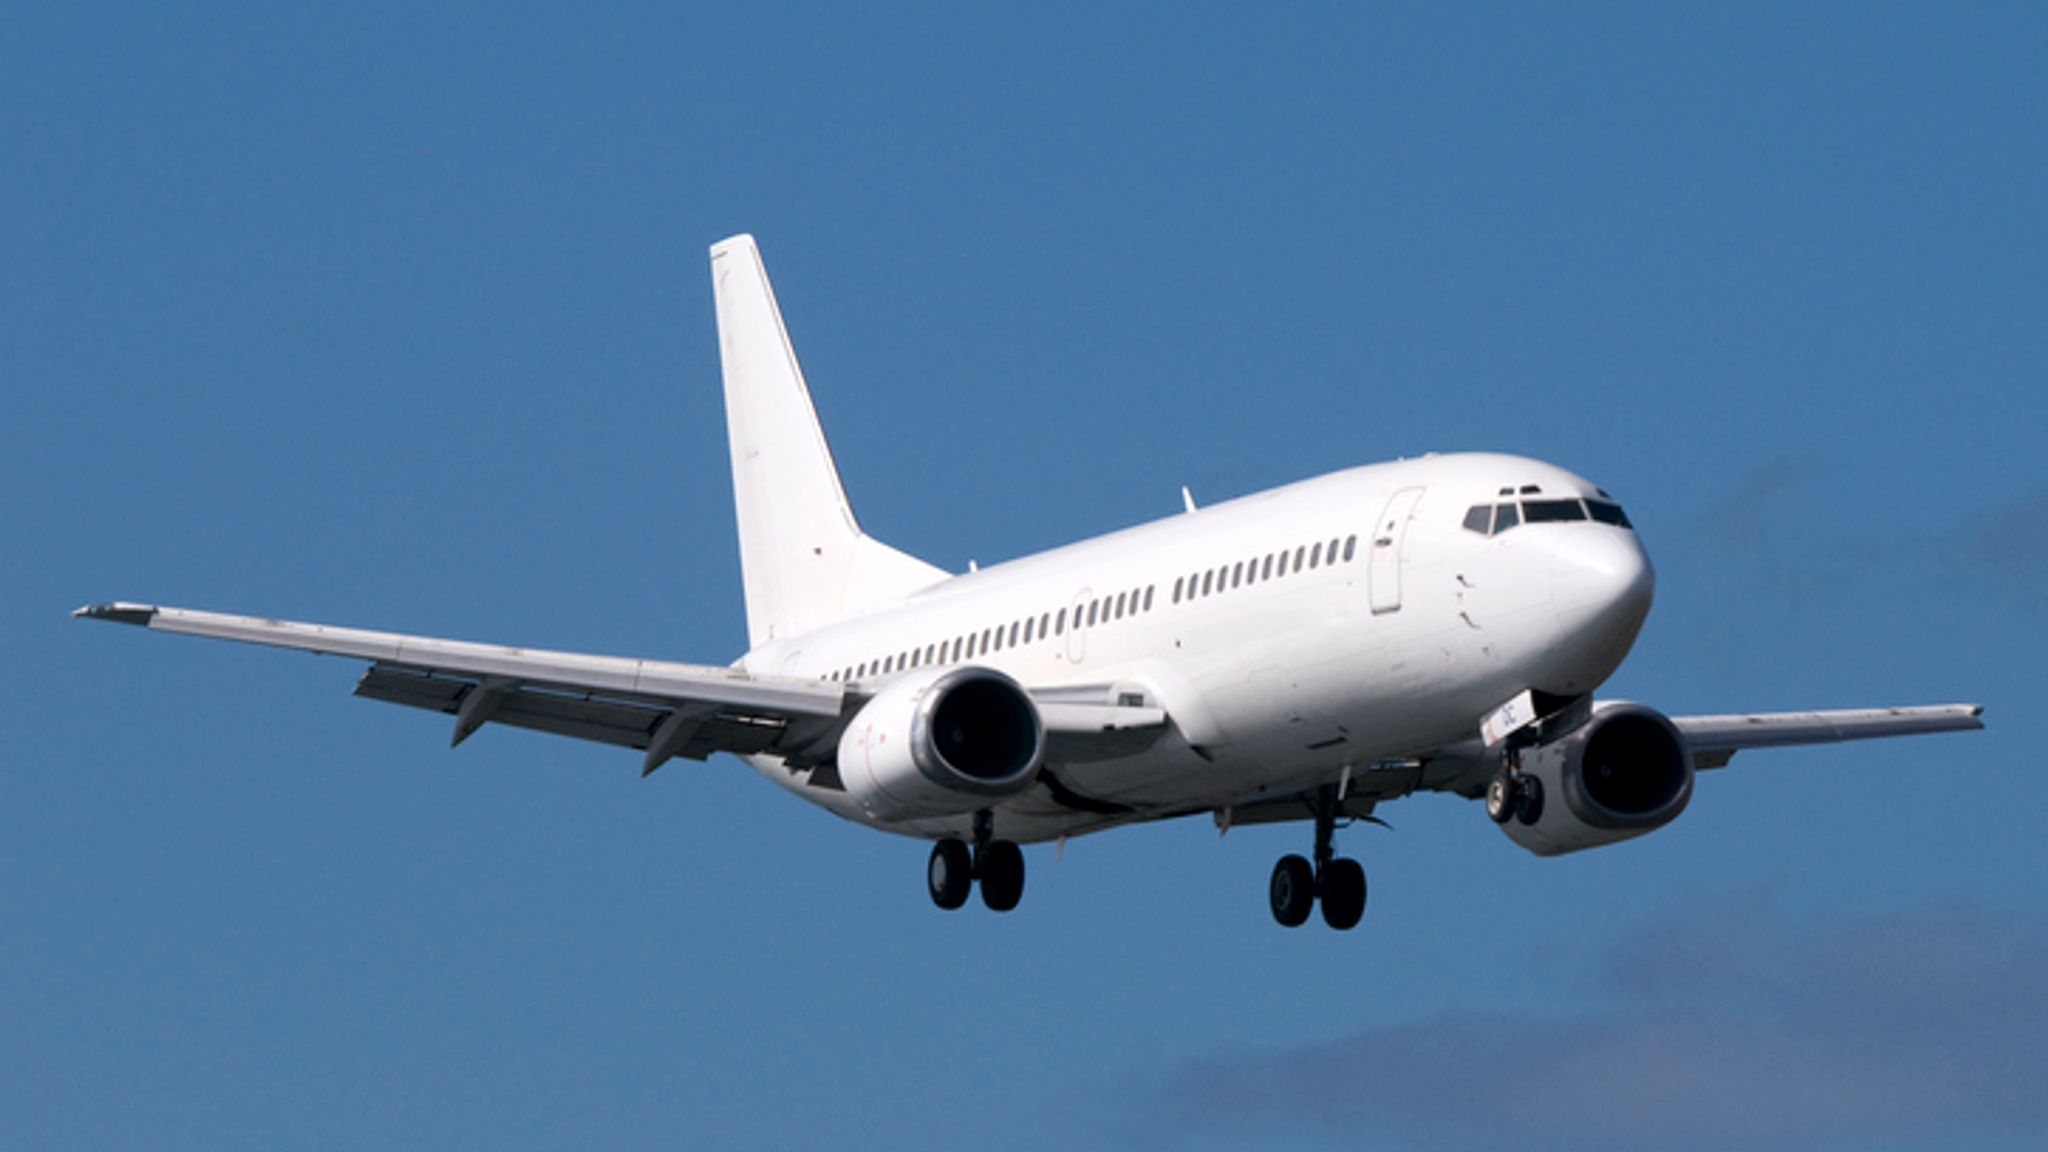
\includegraphics[width=\textwidth]{pic/plane.png}
        \end{column}
    \end{columns}

    \hfill \break
    \hfill \break

    Critical Real-Time Systems are expected to finish on time, otherwise the disaster could happen. This often requires special hardware and software that can be analyzed for timing properties.
    
\end{frame}


\begin{frame}{WCET Analysis}
    \begin{columns}
        
    \column{0.4\textwidth}

    \textbf{W}orst \textbf{C}ase \textbf{E}xecution \textbf{T}ime Analysis:
    \begin{itemize}
        \item Hardware + Software $\downarrow$
        \item Upper bound for execution time?
    \end{itemize}


    \begin{block}{}
        Using abstract execution models. Split analysis into phases related to SW and HW parts.
    \end{block}

    \column{0.6\textwidth}

    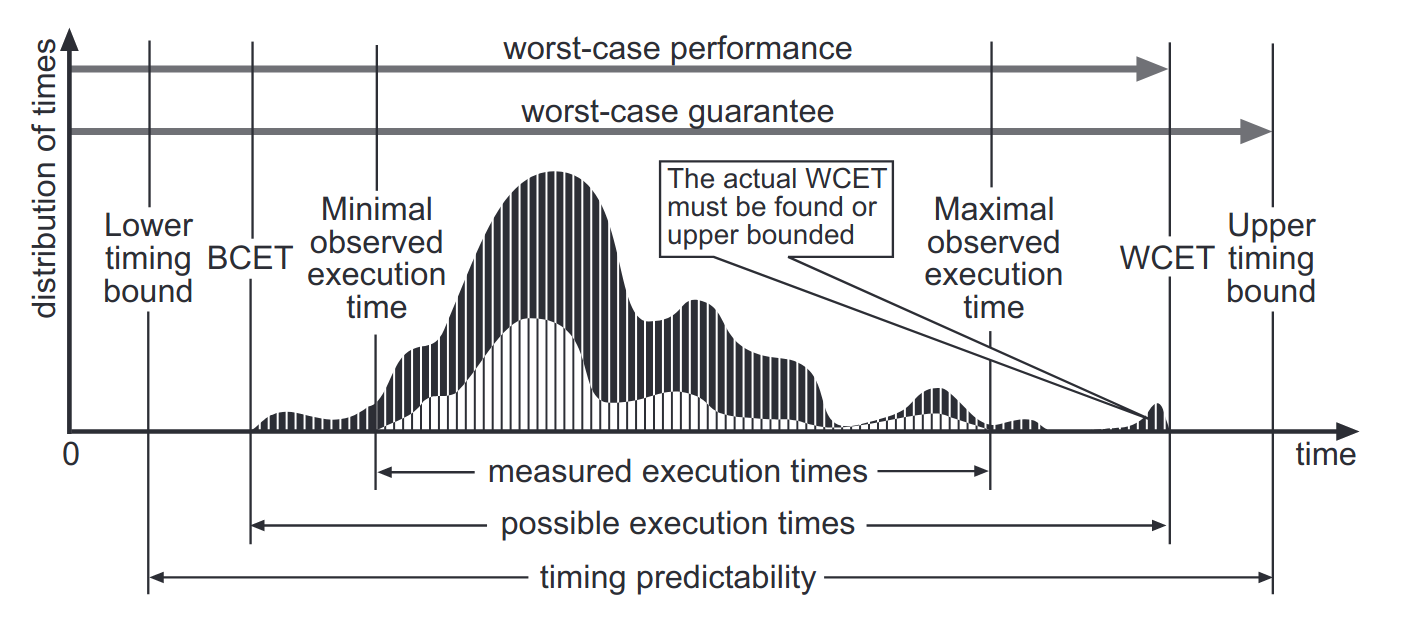
\includegraphics[width=1\textwidth]{pic/timing-distribution.png}

    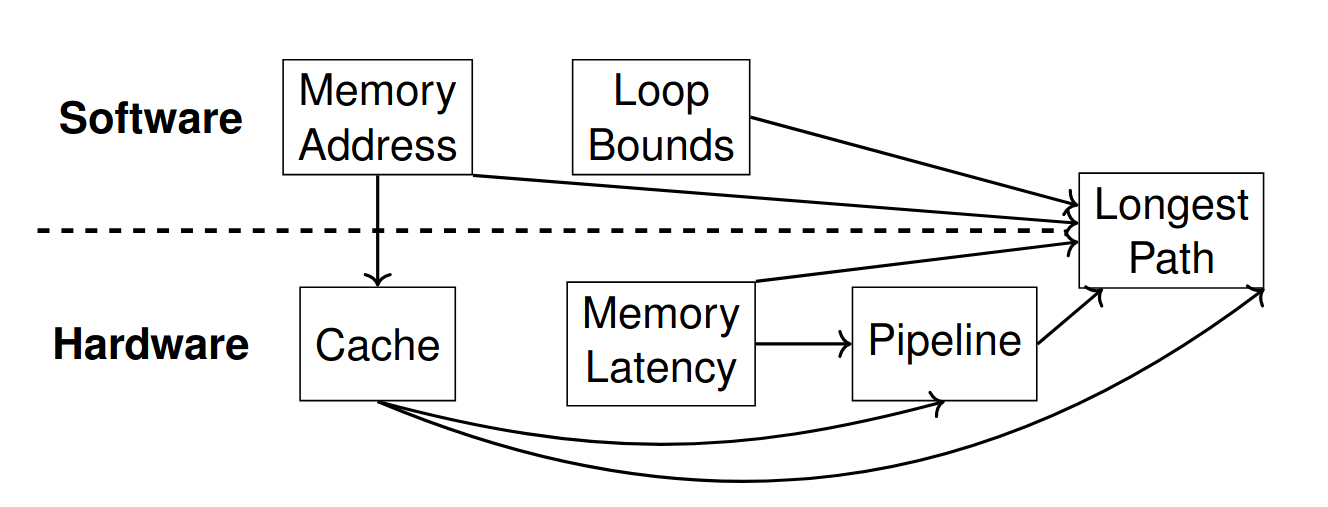
\includegraphics[width=1\textwidth]{pic/wcet-deps.png}

    \end{columns}
\end{frame}

\begin{frame}{Timing Anomalies}
    \begin{block}{Timing Anomaly (TA)}
        When a local speedup leads to a global slowdown.
    \end{block}

    \begin{exampleblock}{Example}
        Faster completion of $A$ leads to a slowdown of the whole trace. 
    \end{exampleblock}

    \begin{columns}
    \column{0.4\textwidth}
        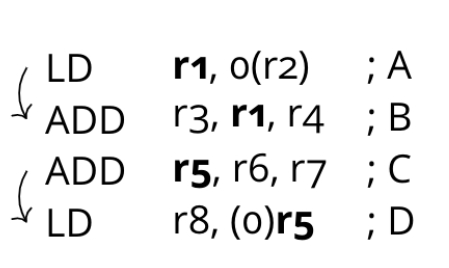
\includegraphics[width=1\textwidth]{pic/first-TA-ex-input.png}
    \column{0.6\textwidth}
        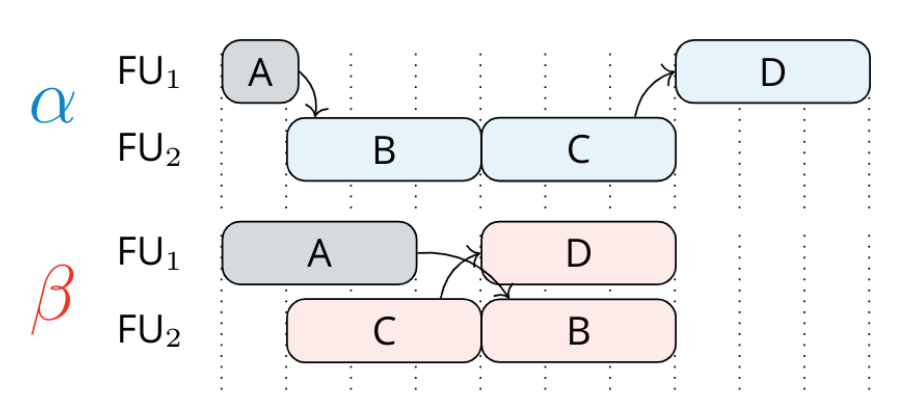
\includegraphics[width=1\textwidth]{pic/first-TA-ex-trace.png}
    \end{columns}
    
\end{frame}
    
\section{Hardware}

\begin{frame}{OoO Multiscalar Pipeline}
    Processor:
    \begin{itemize}
        \item \textbf{Pipelined:} Divided into consecutive stages
        \item \textbf{Multiscalar:} Fetch multiple instruction in the same time
        \item \textbf{Out-of-Order:} Execution order dictated by instruction dependencies
    \end{itemize}


    \begin{columns}
    \column{0.5\textwidth}
        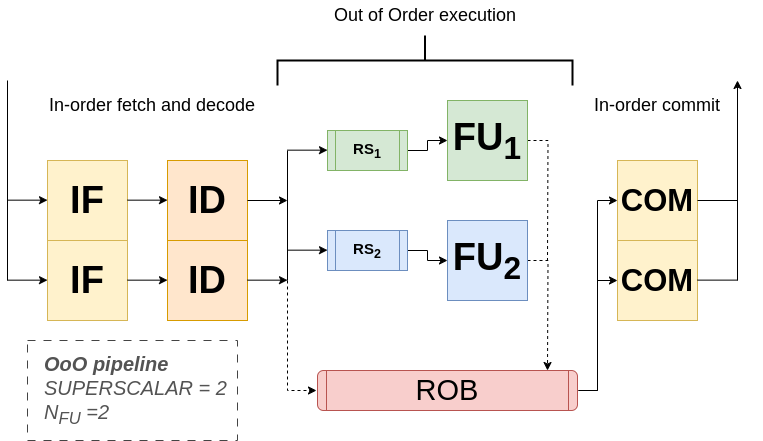
\includegraphics[width=\textwidth]{pic/ooo-pipeline.png}
    \column{0.5\textwidth}
        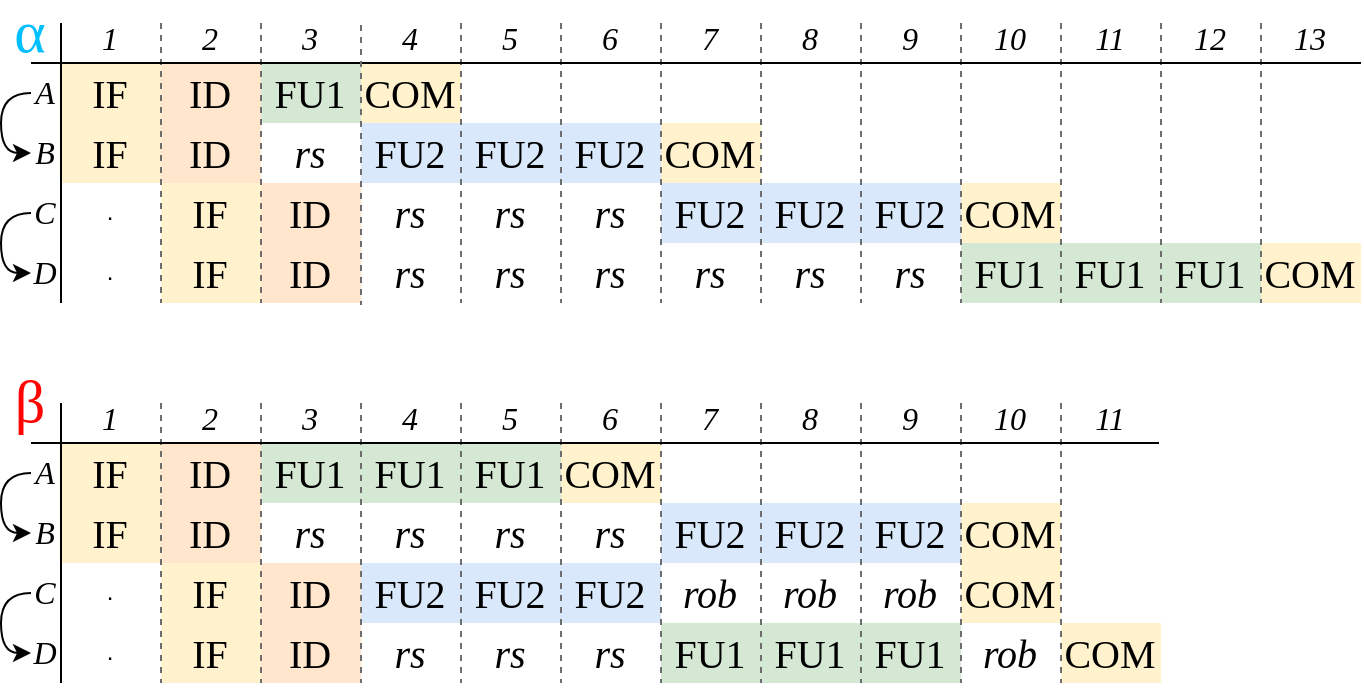
\includegraphics[width=\textwidth]{pic/multiscalar_ta.png}
    \end{columns}

\end{frame}

\begin{frame}{Branch Prediction}
    \begin{itemize}
        \item Branch target unknown until resolved.
        \item Predict next address and execute speculatively.
        \item On misprediction: jump to correct address.
    \end{itemize}
    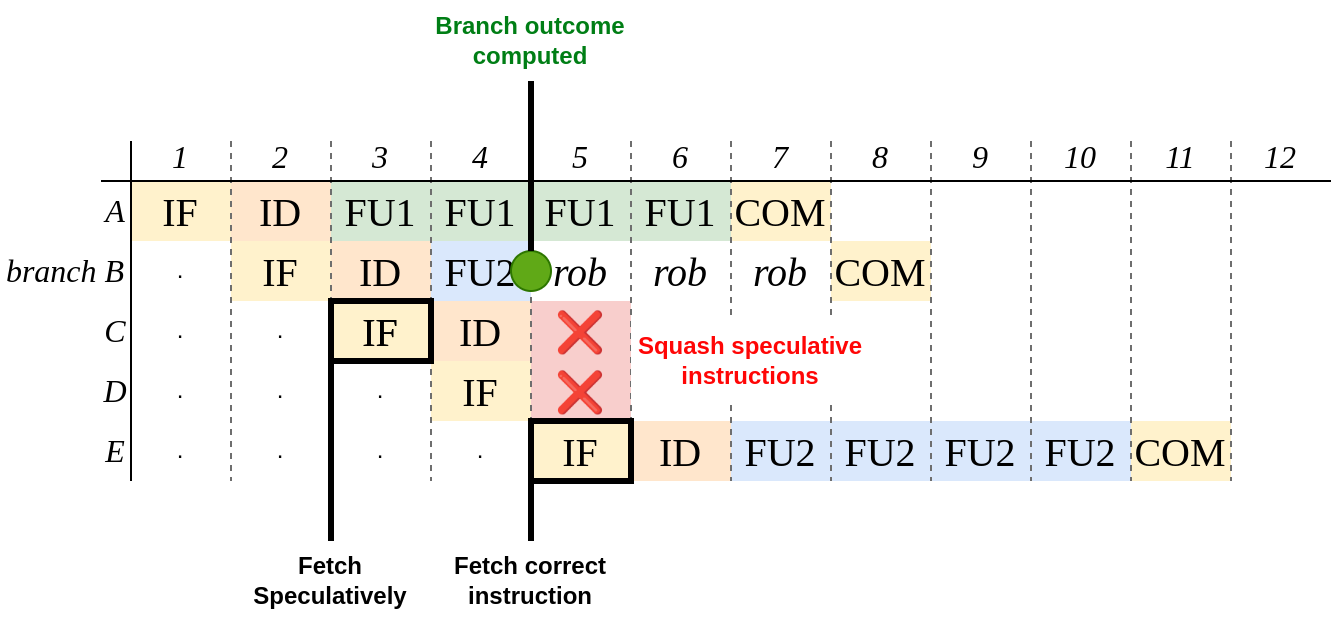
\includegraphics[width=\textwidth]{pic/bp-demo.png}
\end{frame}

\begin{frame}{Branch Prediction: possible implementations}
    \begin{columns}
    \column{0.5\textwidth}

    \begin{block}{Additional Hardware}
        \begin{itemize}
            \item Pattern History Table (PHT)
            \item Branch Target Buffer (BTB)
        \end{itemize}
    \end{block}

    \begin{exampleblock}{Example: 2-bit counter}
        For each branch store a 4-state automaton in PHT
    \end{exampleblock}

    \column{0.5\textwidth}

    \begin{block}{Strategies}
        \textbf{Static:} always take, never take, take backwards. \\        
        \textbf{Dynamic:} 
        \begin{itemize}
            \item 1 or 2-Bit Counter
            \item Global or Local History
            \item Global share
        \end{itemize}
        and more...
    \end{block}

    \end{columns}

    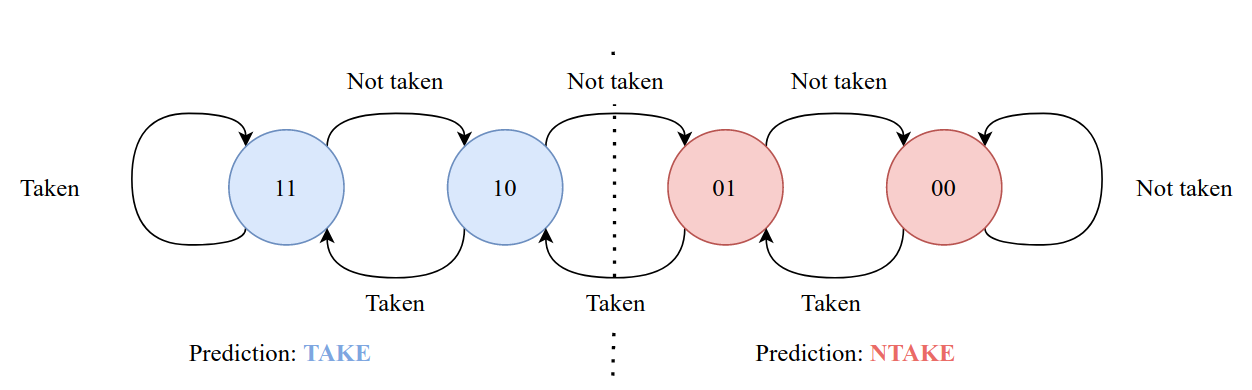
\includegraphics[width=0.9\textwidth]{pic/two-bit-counter.png}

\end{frame}

\section{Timing Anomalies}

\begin{frame}{Formal Definition?}
    \textbf{How do we formally define a TA?}

    \begin{block}{Some existing definitions}
        \begin{itemize}
            \item Step Heights (by Gebhard et al.)
            \item Step-functions Intersections (by Cassez et al.)
            \item Component Occupation (by Kirner et al.)
            \item Instruction Locality (by Reineke et al.)
            \item Event Time Dependency Graph (by Binder et al.)
        \end{itemize}
    \end{block}
\end{frame}

\begin{frame}{Step Heights by Gebhard et al.}
    \begin{block}{Definition}
        TA = one instruction executes faster, the instruction after -- slower
    \end{block}

    \includegraphics<1>[width=\textwidth]{pic/step-height-good.png}

    \begin{alertblock}<2>{Counterexample!}
        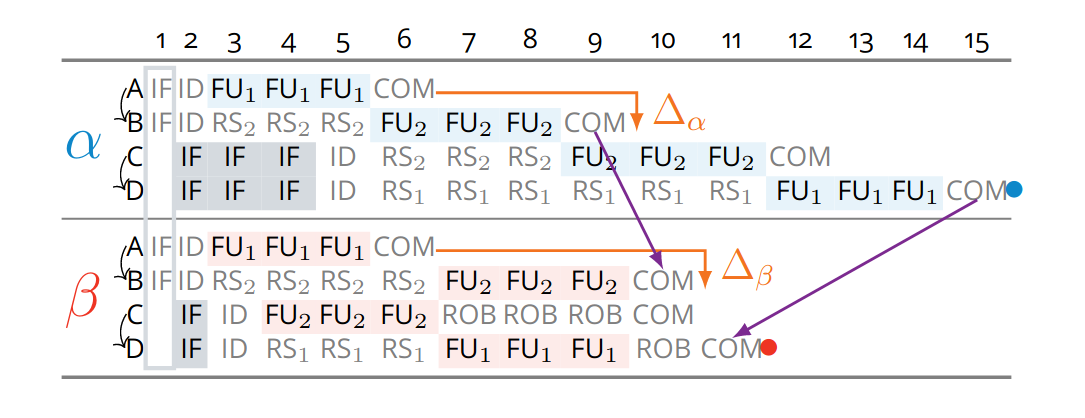
\includegraphics[width=0.8\textwidth]{pic/step-height-bad.png}
    \end{alertblock}
\end{frame}

\begin{frame}{Step Function Intersections by Gebhard et al.}
    \begin{block}{Definition}
        Step Function = instruction $\rightarrow$ its completion time
        TA = intersection of step functions of 2 traces
    \end{block}

    \only<1>{
        \begin{columns}
        \column{0.6\textwidth}
            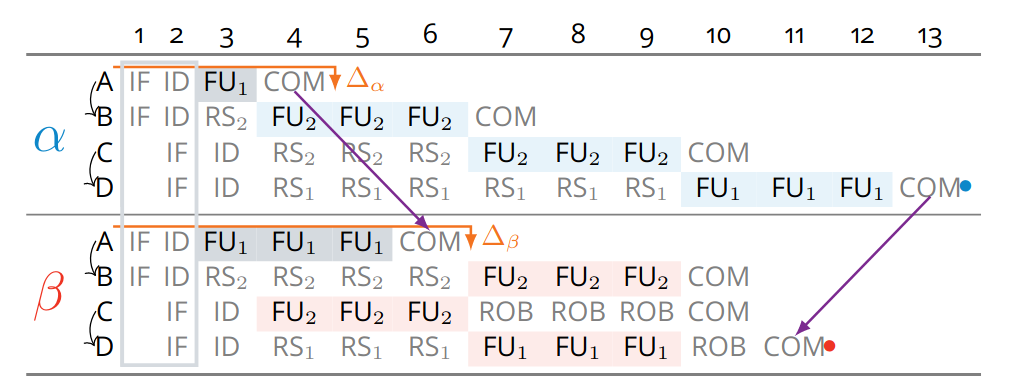
\includegraphics[width=\textwidth]{pic/step-height-good.png}
        \column{0.4\textwidth}
            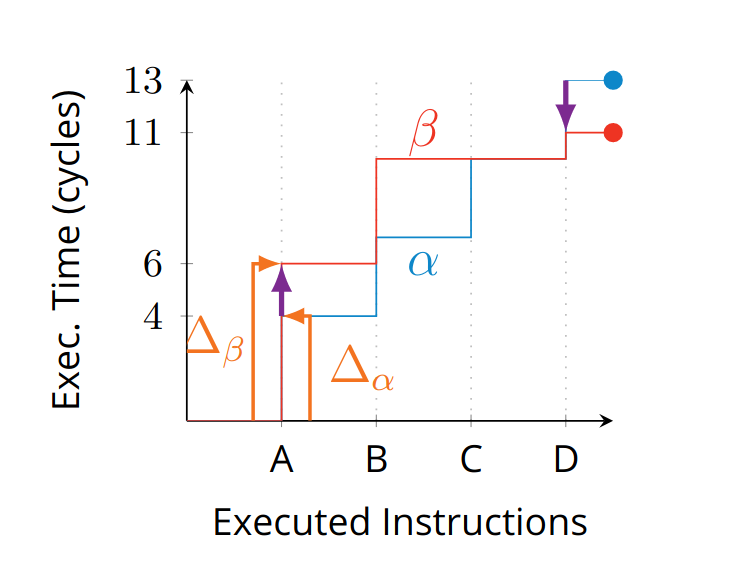
\includegraphics[width=\textwidth]{pic/step-functions.png}
    \end{columns}
    }
    
    \only<2>{
        \begin{alertblock}{Counterexample!}
            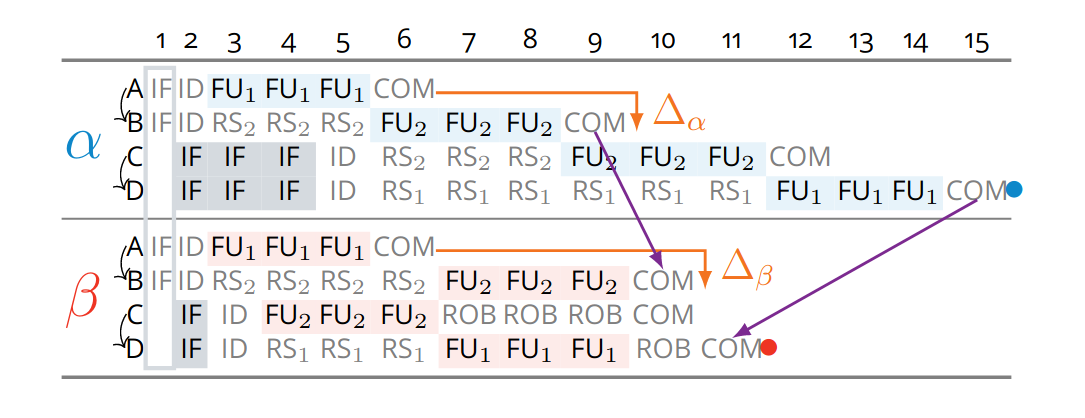
\includegraphics[width=0.9\textwidth]{pic/step-functions-bad.png}
        \end{alertblock}
    }   
\end{frame}

\begin{frame}{Event Time Dependency Graph by Binder et al.}
    \begin{block}{3 Components}
        \only<1> {
            \begin{enumerate}
                \item Latency
                \item Delay
                \item Causality
            \end{enumerate}
        }
        \only<2> {
            \begin{enumerate}
                \item \textbf{Latency}
                \item Delay
                \item Causality
            \end{enumerate}
        }
        \only<3> {
            \begin{enumerate}
                \item Latency
                \item \textbf{Delay}
                \item Causality
            \end{enumerate}
        }
        \only<4> {
            \begin{enumerate}
                \item Latency
                \item Delay
                \item \textbf{Causality}
            \end{enumerate}
        }
    \end{block}

    \includegraphics<1>[scale=0.17]{pic/binder-def-1.png}
    \includegraphics<2>[scale=0.17]{pic/binder-def-2.png}
    \includegraphics<3>[scale=0.17]{pic/binder-def-3.png}
    \includegraphics<4>[scale=0.17]{pic/binder-def-4.png}
\end{frame}

\begin{frame}
    \begin{block}{Goal}
        Develop a consistent TA definition applicable for branch prediction.
    \end{block}
\end{frame}

\section{Contribution}

\begin{frame}{Research Plan}
    \begin{itemize}
        \item \textbf{Goal:} Systematically investigate TAs induced by branch predictors.
        \item Manual construction of examples is inefficient and error-prone.
        \item \textbf{Approach:} Develop a tool to automatically or semi-automatically generate and validate relevant examples.
        \item Use the tool to:
        \begin{itemize}
            \item Iteratively generate candidate scenarios.
            \item Analyze behavior and assess applicability of Binder et al.'s definition.
            \item Refine the definition based on empirical evidence.
        \end{itemize}
        \item \textbf{Initial step:} Studied and extended Binder et al.'s TLA$+$ framework for branch behavior.
        \item \textbf{Challenge:} TLA+ model had performance and flexibility limitations.
        \item \textbf{Solution:} New the framework in C++.
    \end{itemize}
\end{frame}

\begin{frame}{Ad-hoc C++ Model Checker}
    \begin{itemize}
        \item Written in C++.
        \item Simple and flexible input format.
        \item Supports speculative execution.
        \item Faster than TLA$+$ implementation (milliseconds instead of seconds).
        \item 3 operation modes:
        \begin{enumerate}
            \item Interactive manual mode.
            \item State space exploration.
            \item Randomized search.
        \end{enumerate}
    \end{itemize}
\end{frame}

\begin{frame}{Input Format}

\begin{itemize}
    \item Each branch instruction is followed by \textbf{misprediction region} -- sequence of instruction representing the wrong branch.
    \item A pair of traces is generated from a single input.
\end{itemize}

\begin{columns}
    \column{0.4\textwidth}
        \begin{tabular}{rr|ccc}
         &  & Res & Dep. & Lat. \\ \hline
        \textit{A} &  & FU1 &  & $4$ \\
        \textit{*B} &  & FU2 & $\{A\}$ & $1$ \\
        & \textit{C} & FU2 &  & $4$ \\
        & \textit{D} & FU2 &  & $4$ \\
        \textit{E} &  & FU2 &  & $4$ \\
        \end{tabular}

    \column{0.6\textwidth}
        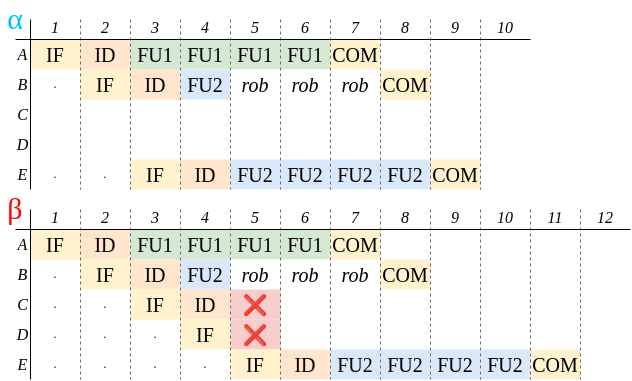
\includegraphics[width=\textwidth]{pic/mispred-intro.png}
\end{columns}

\end{frame}

\begin{frame}{Branch TA}
    Correct prediction leads to a longer execution time.

    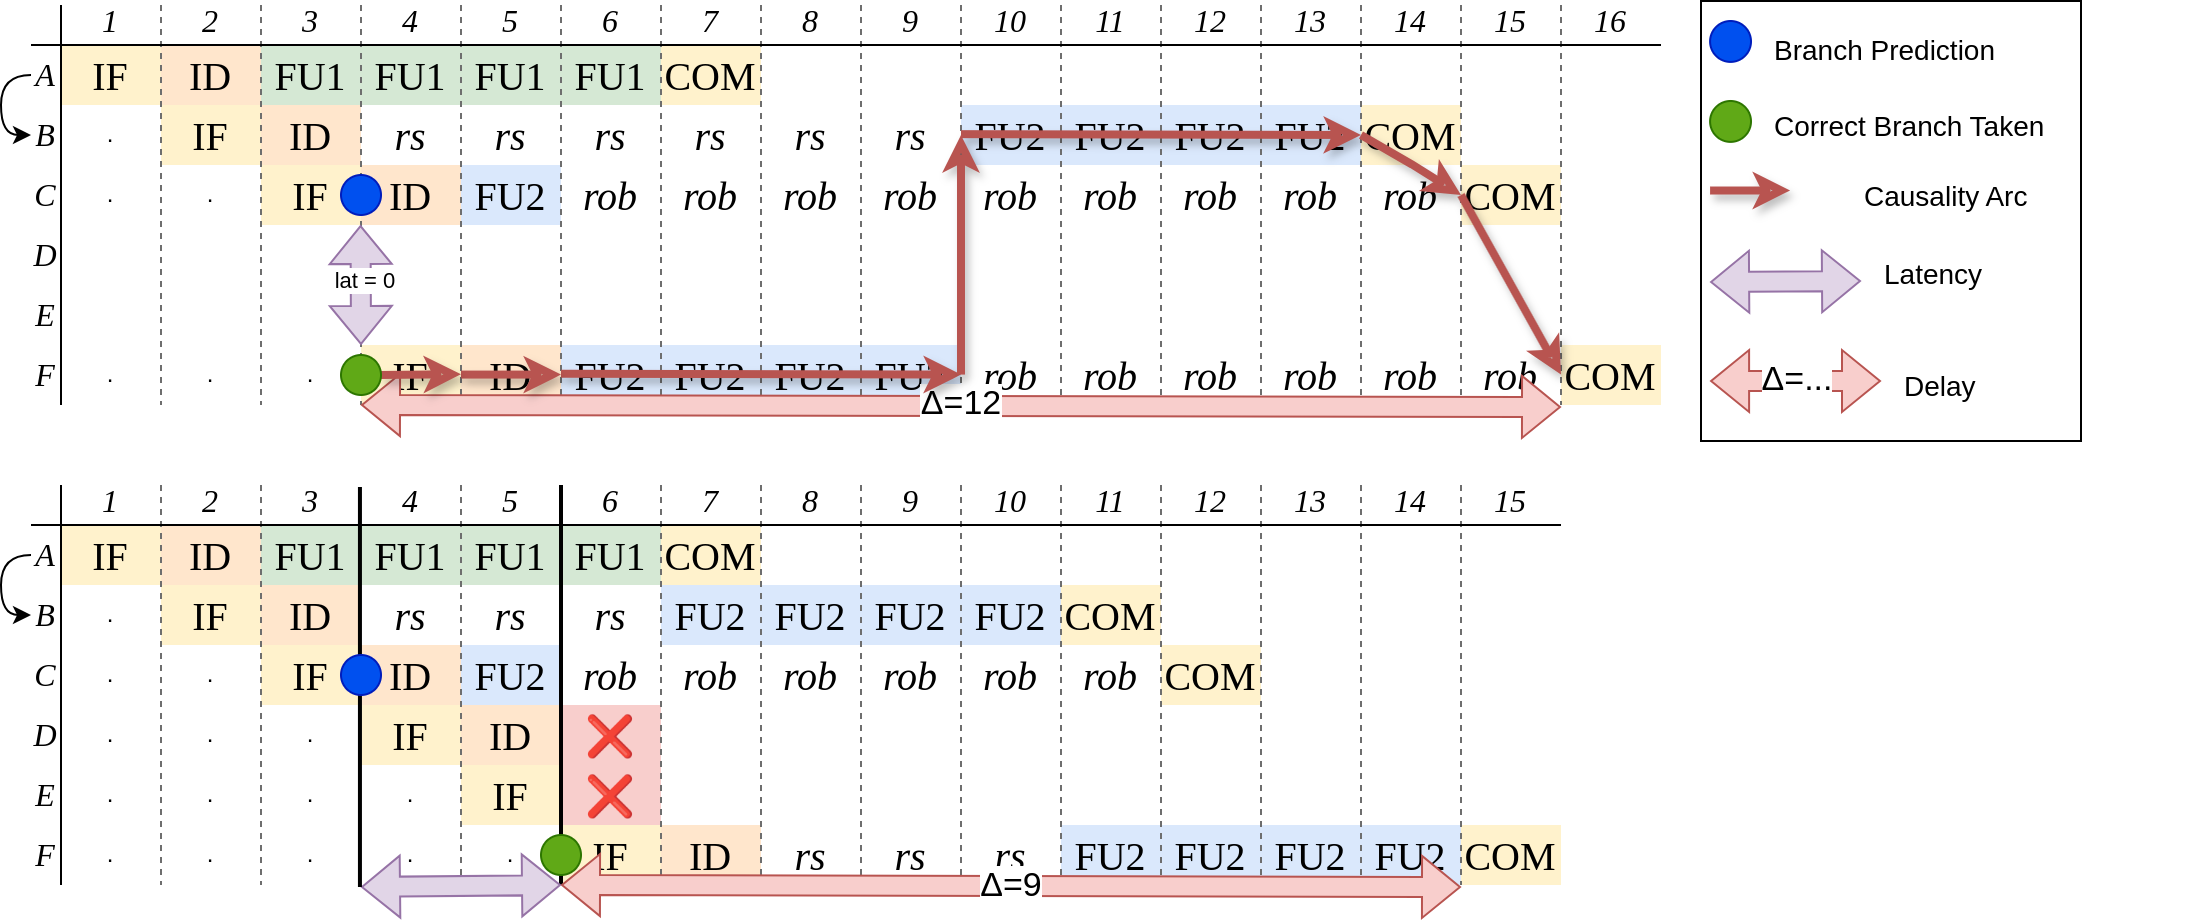
\includegraphics[width=0.8\textwidth]{pic/simple-branch-ta-analyzed.png}

    \begin{block}{New Latency}
        Between "branch prediction" and "correct branch taken" events.
    \end{block}

    Binder's causality rules are applicable.
\end{frame}


\begin{frame}{Early FU Release}
    How to define causality if execution in FU is aborted by squashing?

    \begin{block}{Assumption 1}
        If FU is released as the result of squashing, the FU release of corresponding branch is causal to FU release of the squashed instruction.
    \end{block}

    \begin{block}{Assumption 2}
        The FU acquisition is always causal to the respective FU release.
    \end{block}
\end{frame}

\begin{frame}{Early FU Release}
    \begin{itemize}
        \item \textbf{Assumption 1} does not hold.
        \item \textbf{Assumption 2} holds.
    \end{itemize}
    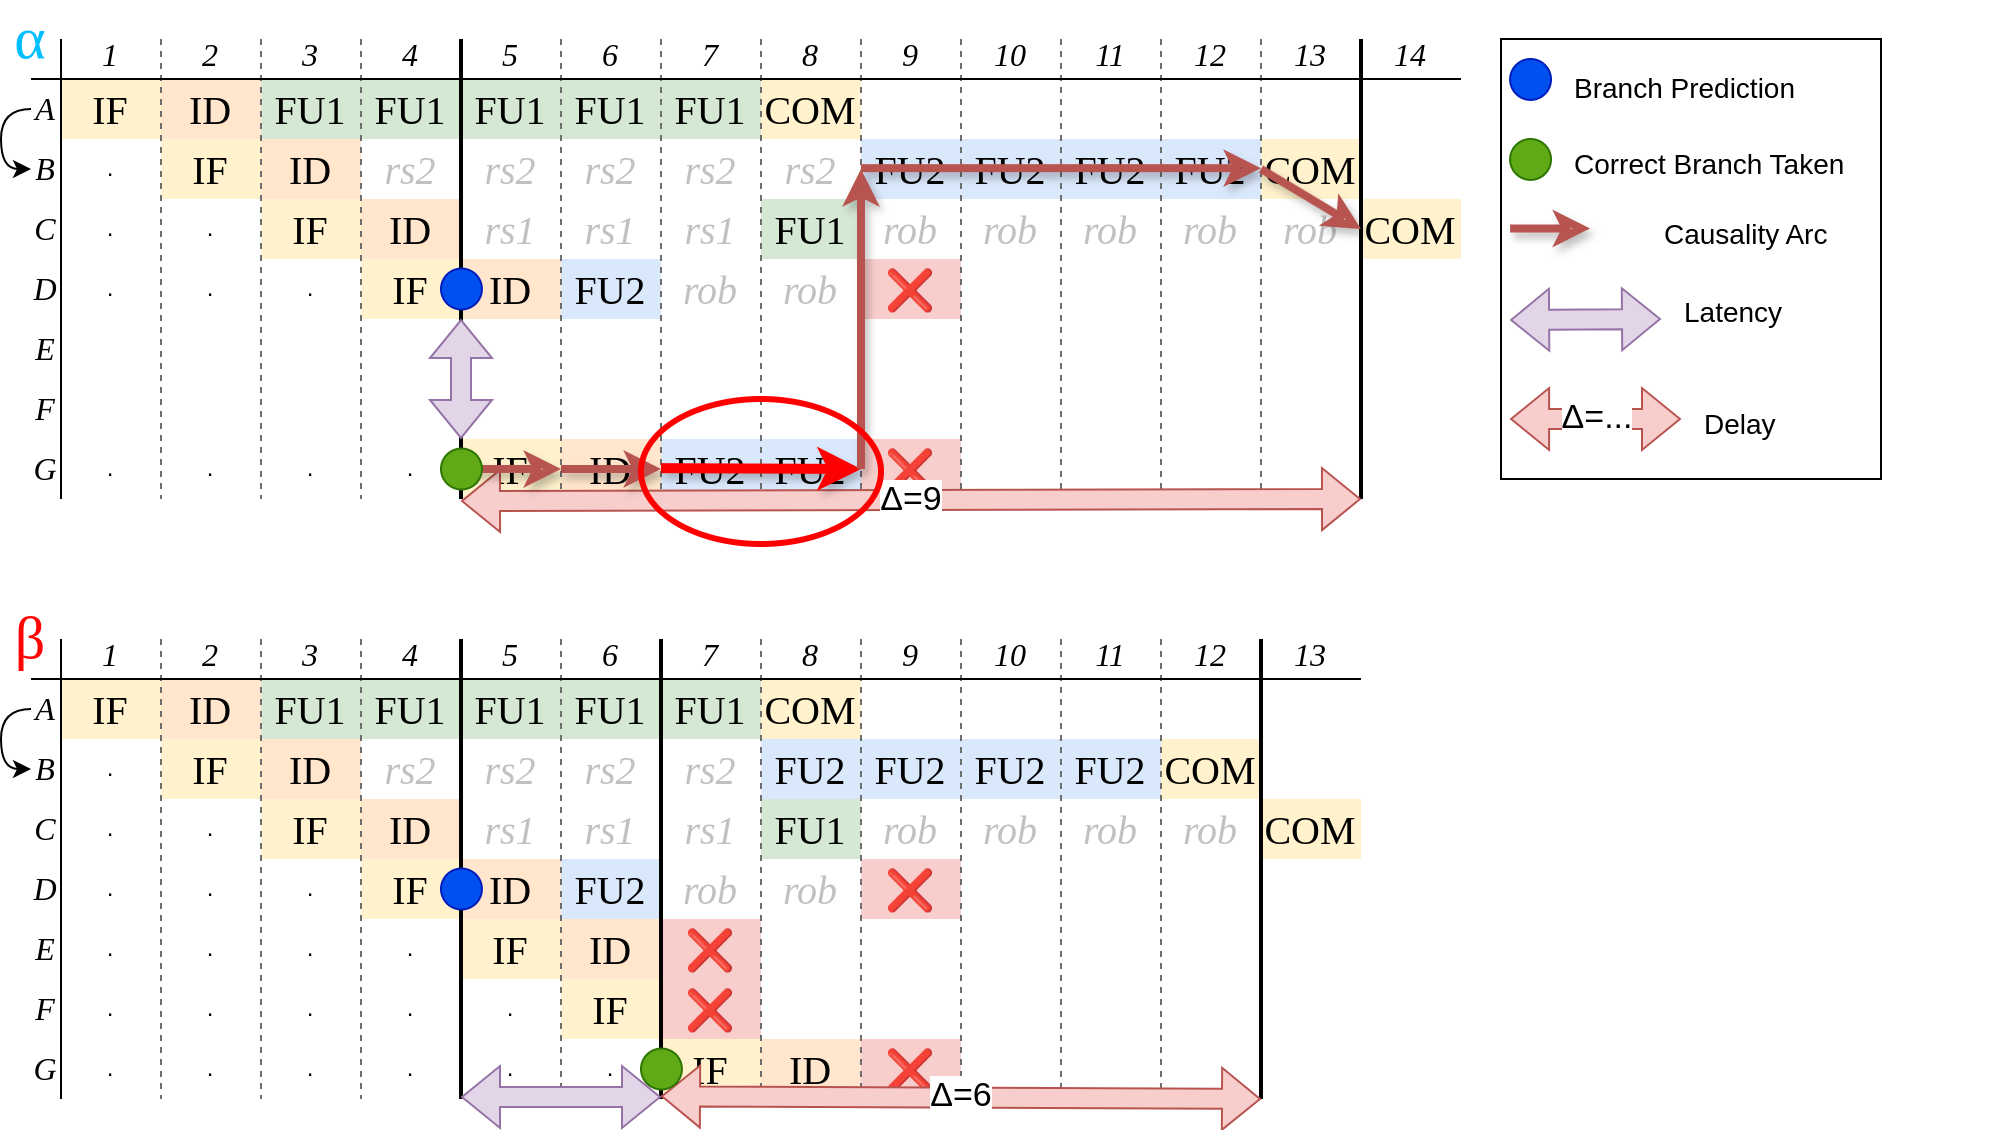
\includegraphics[width=0.9\textwidth]{pic/nested-bp-ta.png}
\end{frame}

\begin{frame}{Early FU Release}
    \begin{itemize}
        \item \textbf{Assumption 1} holds.
        \item \textbf{Assumption 2} does not hold.
    \end{itemize}
    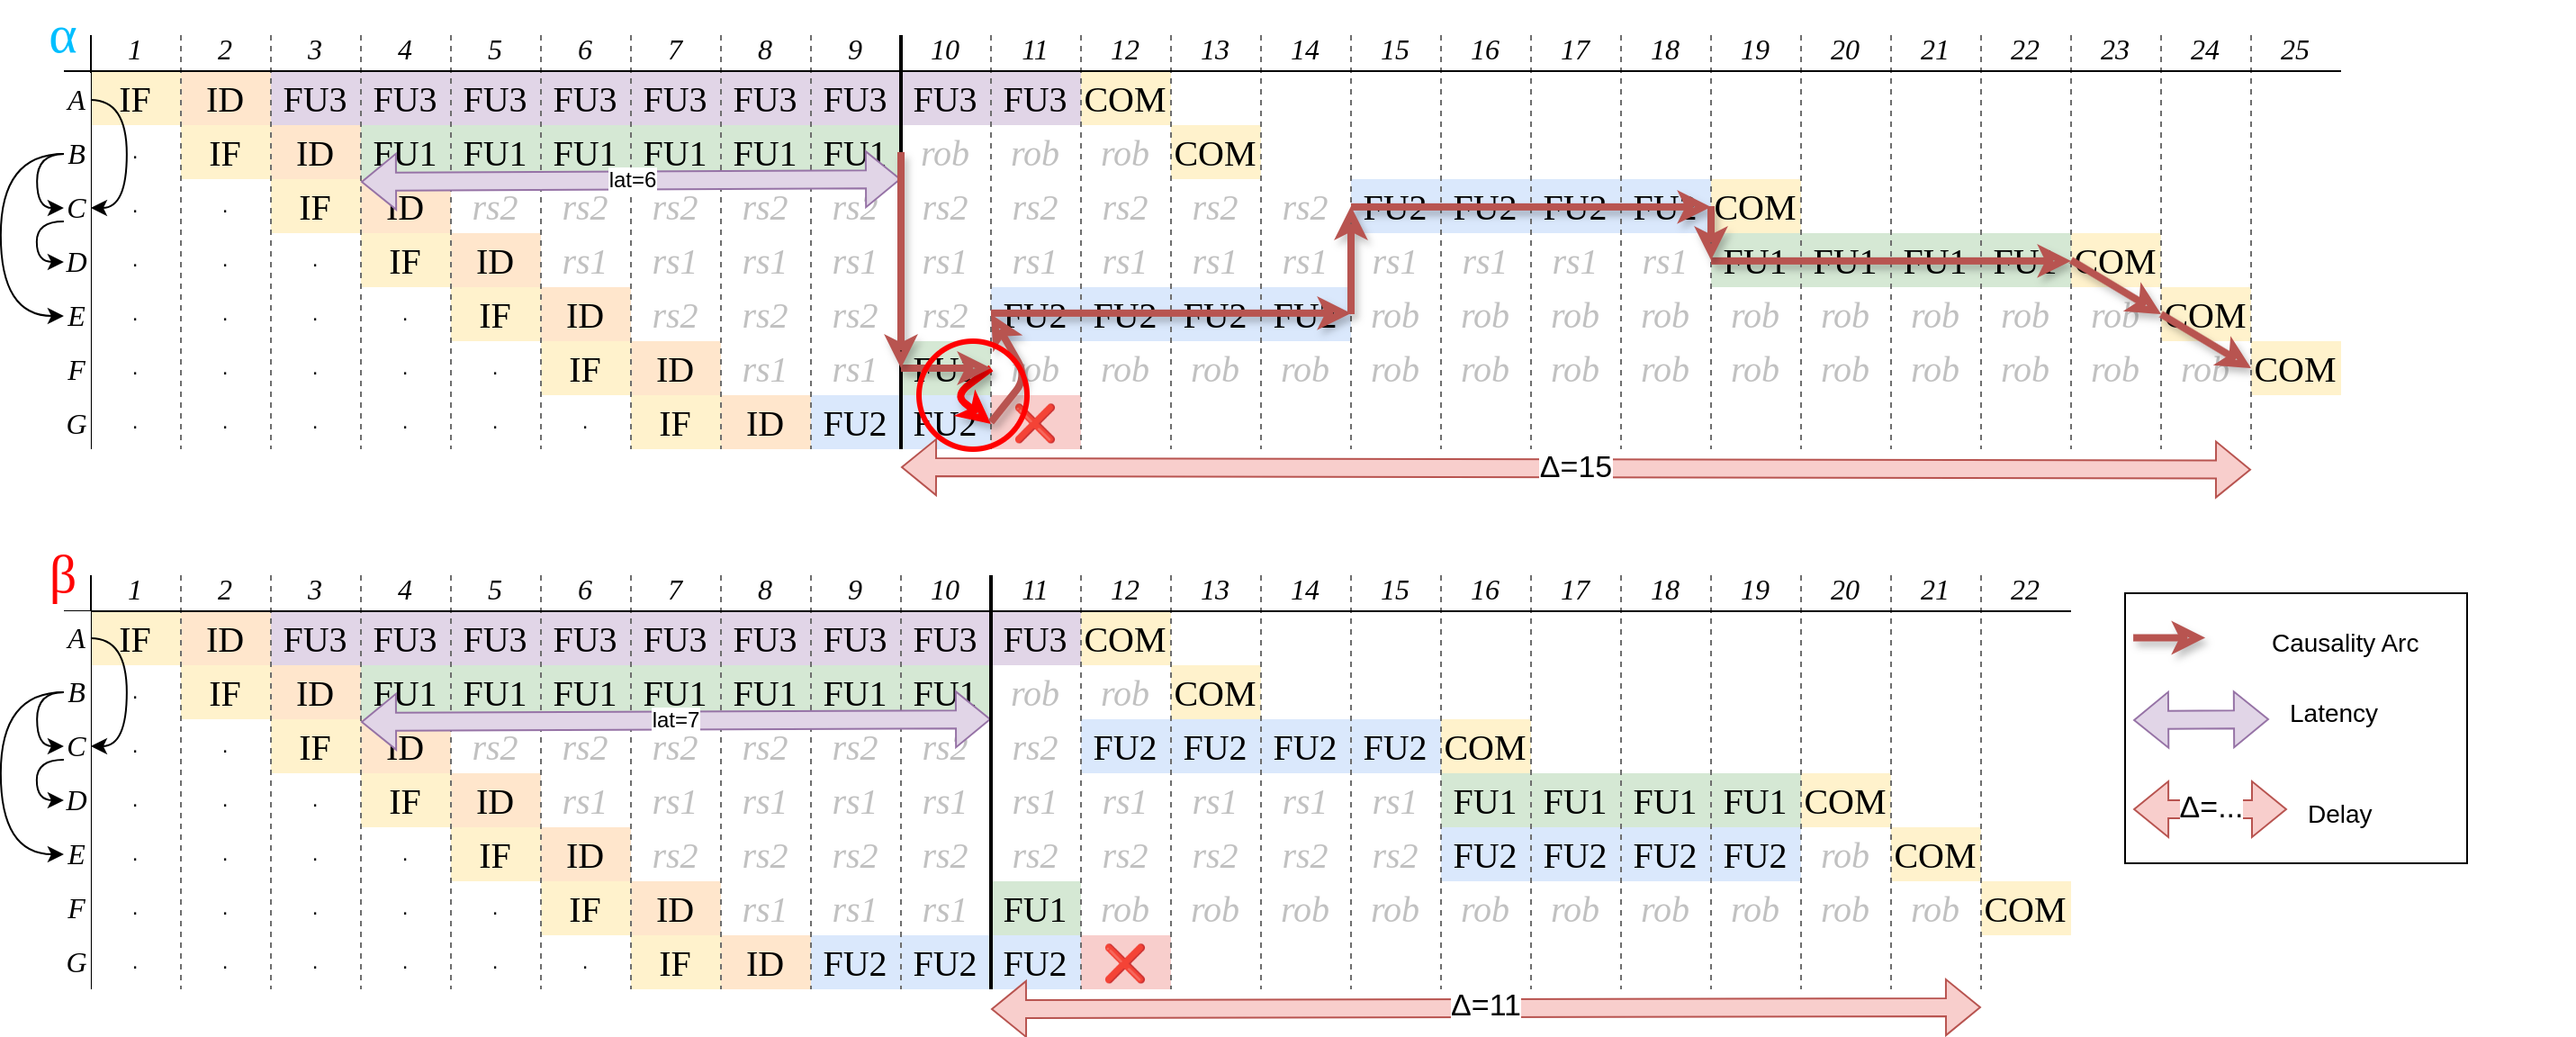
\includegraphics[width=\textwidth]{pic/lat-mispred.png}
\end{frame}

\begin{frame}{Gap Problem}
    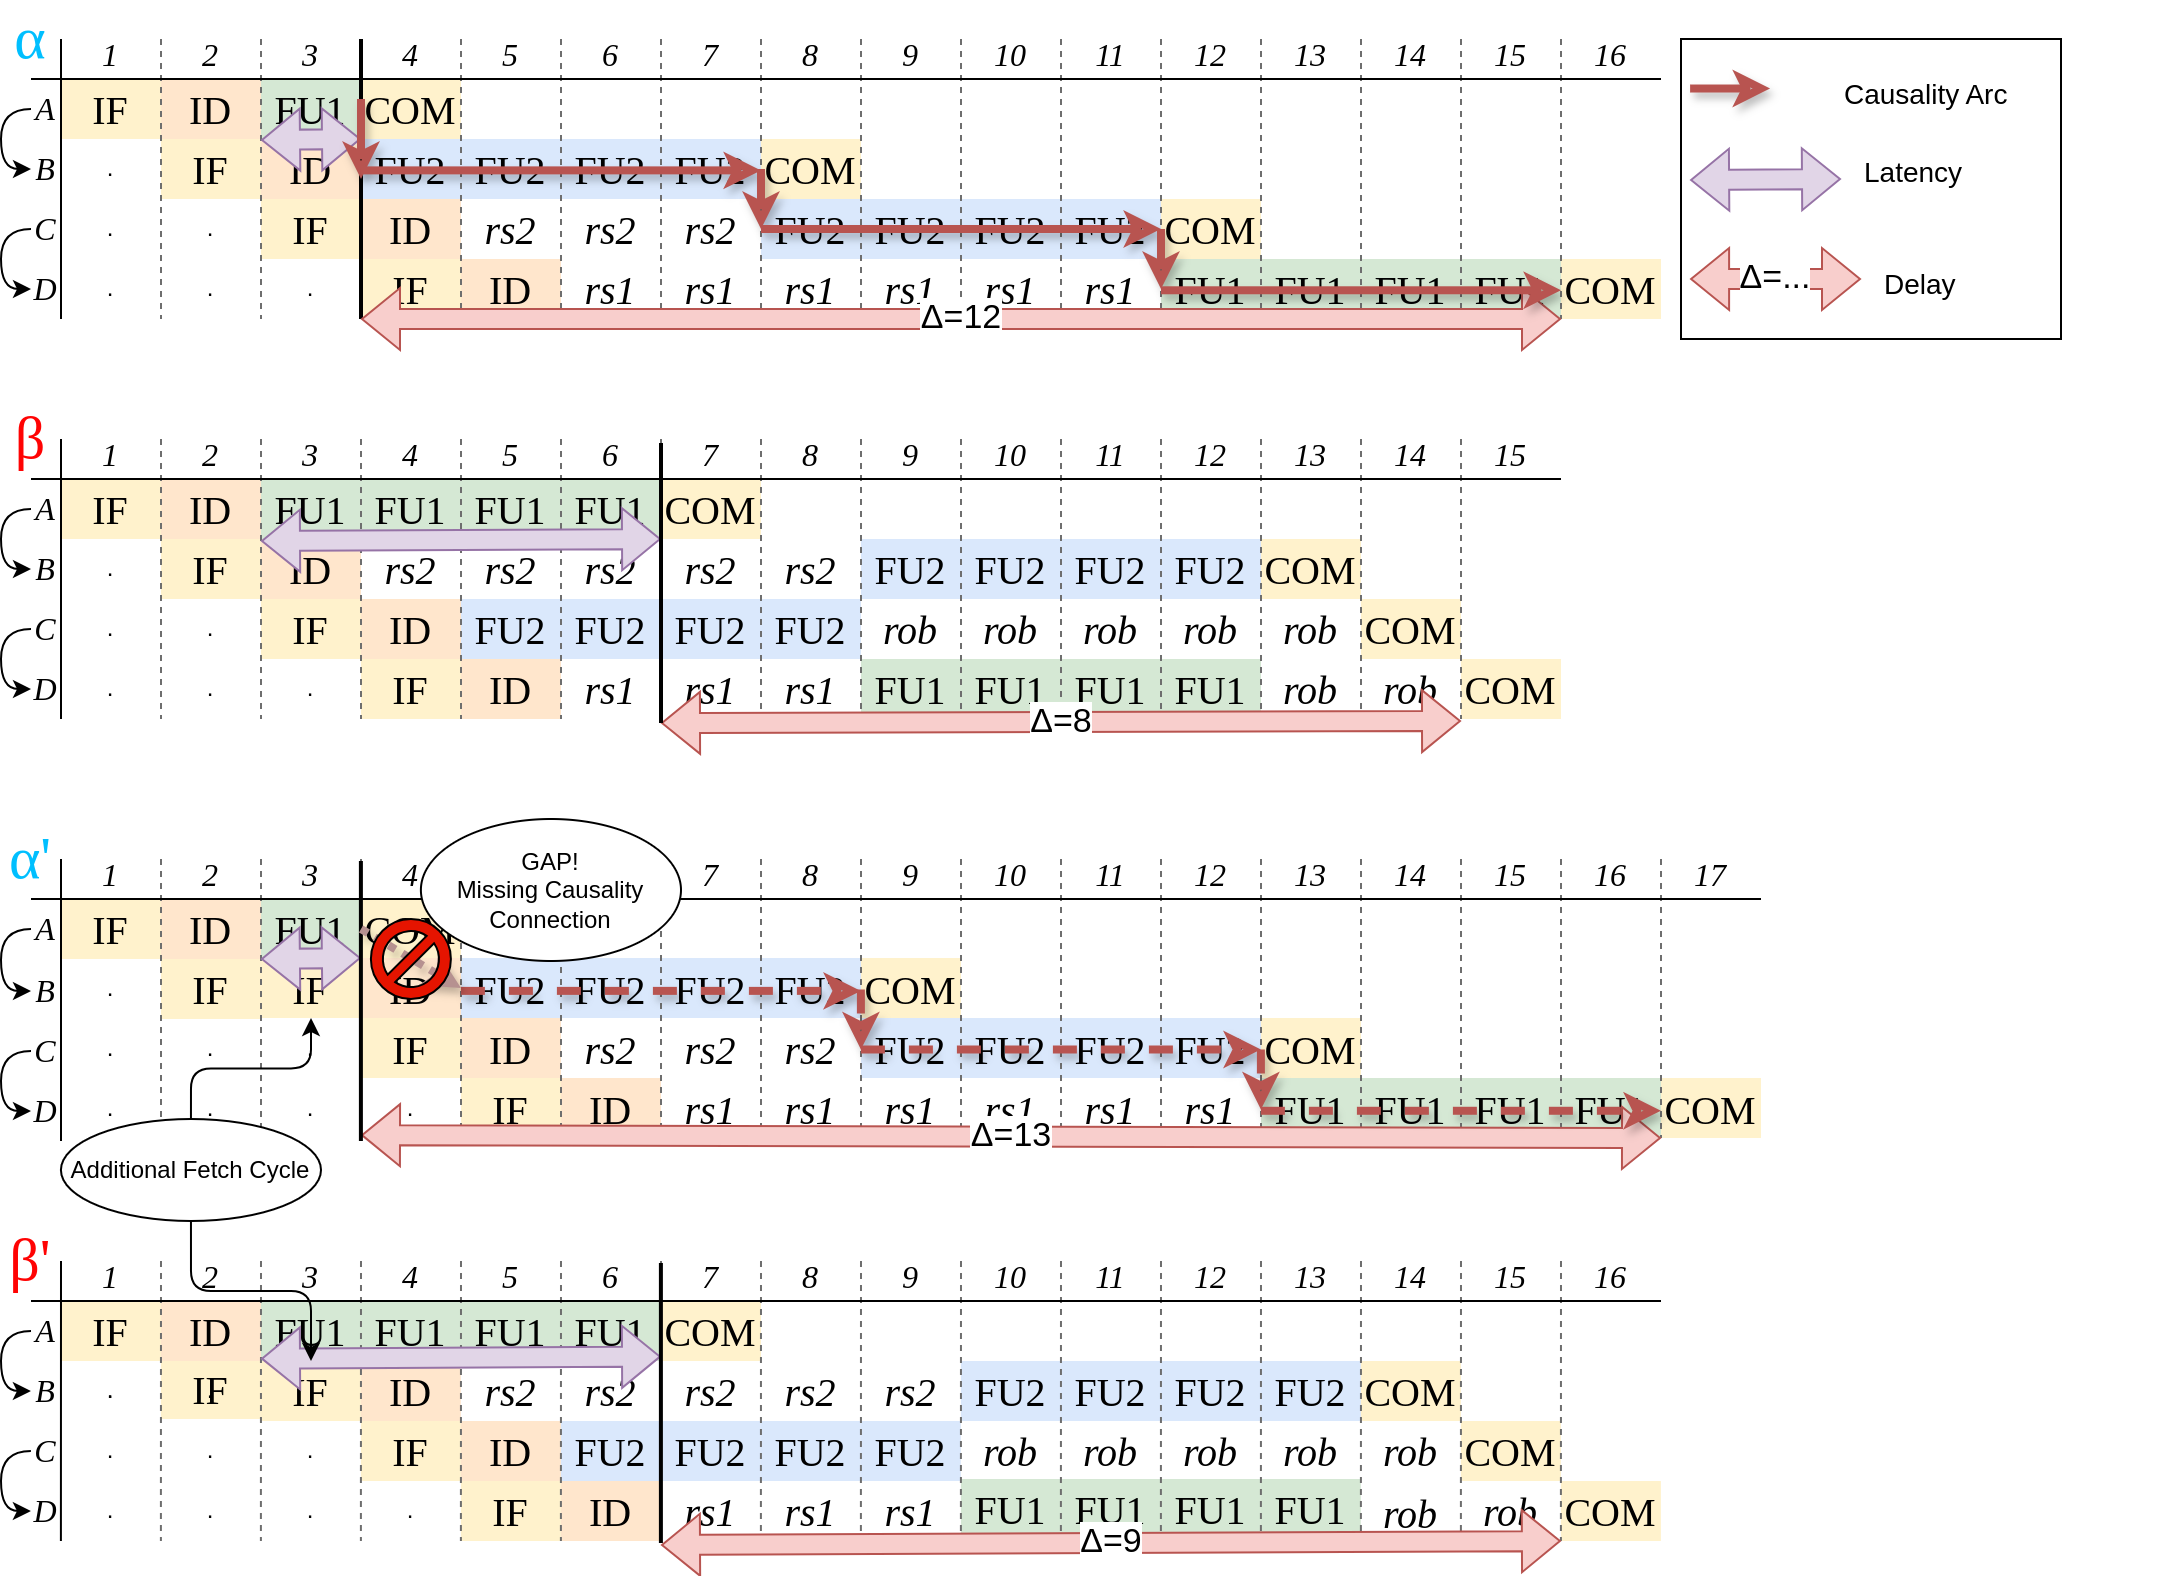
\includegraphics[width=0.9\textwidth]{pic/gap-problem.png}
\end{frame}

\begin{frame}{Results}
    \begin{itemize}
        \item The definition of Binder et al. can be applied in branch prediction context with minimal adjustments.
        \item Sometimes it is not evident which rule to use.
        \item Initial definition suffers from a gap problem.
        \item Likely, the problem is with causality itself.
    \end{itemize}
\end{frame}



\section{Conclusion}

\begin{frame}{Conclusion}
    \begin{itemize}
        \item Analyzed existing timing anomaly (TA) definitions; adopted Binder's causality-based approach.
        \item Developed a tool to systematically generate and analyze branch prediction-induced TAs.
        \item Binder's definition is adaptable, but controversial cases and a "gap problem" remain.
        \item Ongoing work: a new causality definition based on event constraints to address these issues.
        \item Future work: study the impact of branch predictor state.
    \end{itemize}
\end{frame}

\end{document}
